\chapter{Methodology}
\label{chap:methodology}

This chapter outlines the specific procedures and activities carried out to develop, test, and analyze the simulation model of the Braess Paradox within Iloilo City’s traffic network.

\section{Research Activities}
\label{sec:research_activities}

As illustrated in Figure \ref{fig:research_activities}, the researchers conducted a series of research activities. The process begins with Data Gathering, where the researchers collected information and parameters necessary for the study. These findings then serve as inputs for the computational modeling phase. Finally, the researchers analyzed the results of the previous phase to identify and evaluate the presence of the Braess Paradox in the Iloilo City network. 

\begin{figure}[H]
    \centering
    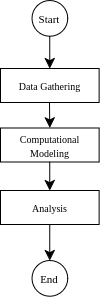
\includegraphics[scale=0.7]{figures/figure-3.png}
    \caption{Research Activities Flowchart} 
    \label{fig:research_activities}
\end{figure}

\section{Data Gathering}
\label{sec:data_gathering}

The researchers identified and mapped the primary highways and intersections based on the DPWH Atlas 2024 for the Iloilo City Network (Department of Public Works and Highways, 2026). 
The scope of the map was also limited strictly to major highways (See Figure~\ref{fig:dpwh_atlas} of Appendix~\ref{app:network_data_files}) 

This process was then categorized into node identification and edge attribution to provide a digital representation of the city’s road infrastructure.  Additionally, Origin-Destination (OD) matrix pairs were identified for defining traffic demand. 

\subsection{Node Identification}
\label{sec:node_identification}

During node identification,  the researchers identified key intersections within the Iloilo City network utilizing Google Maps (Google, n.d). These intersections served as nodes for the network. For each node, specific metadata was collected. The metadata structure can be found in Listing~\ref{lst:intersection_data} of Appendix~\ref{app:source_codes}.

Here, ``\texttt{id}'' stands as a unique identifier for programmatic referencing, ``\texttt{latitude}'', and ``\texttt{longitude}'' as the precise geospatial coordinates of the intersection.


\subsection{Edge Attribution}
\label{sec:edge_attribution}

Road segments connecting the identified nodes were defined as edges. Specific roadway characteristics were then gathered for each edge. The structure can be found in Listing~\ref{lst:road_data} of Appendix~\ref{app:source_codes}.

Here, ``\texttt{distance}'' serves as the physical length of the road from point $A$ to point $B$, in meters, and used as a primary parameter for calculating travel time and cost functions. ``\texttt{lanes}'' as the number of available lanes, which influences the capacity of the road, and ``\texttt{one\_way}'' as a boolean constraint applied to each edge to represent the flow of traffic accurately.

\subsection{OD Matrix Pair Identification}
\label{sec:pair_identification}

The researchers gathered data for OD matrix pairs based on the Master Plan Study on the Strategic Road Network Development project report (Japan International Cooperation Agency, 2003). These OD matrix pairs define the volume and direction of travel demand within the Iloilo City network. The demands were derived by the Japan International Cooperation Agency (2003) based on future socio-economic projections for the year 2022 that included the population by city, employment, the vehicle ownership projection, and the Gross Regional Domestic Product (GRDP) of Region VI. The OD pairs in the Iloilo City network were partitioned into sixteen Traffic Analysis Zones (TAZs). 

This socio-economic framework is used as explanatory variables for multi-step demand forecast models: traffic generation or attraction models, trip distribution models, and modal split models. For the traffic generation and attraction model, the employment variables were used to calculate the amount of passenger and cargo trips that each zone will produce and attract. For the modal split, it utilized the projection of vehicle ownership to determine how passenger trips are divided between private vehicles and public transport. It projected the future vehicle ownership rates that were derived from the GRDP growth.  The  first 15 rows and columns of the OD matrix can be found in Table {\ref{tab:od_matrix_15}} of Appendix~\ref{app:network_data_files}
.


\subsection{Annual Average Data Traffic}
\label {sec:aadt}

Annual Average Data Traffic (AADT) is a metric in transportation planning calculated by dividing the total annual vehicular volume on specific road segments by 365 to establish the mean daily traffic flow (Dishin, 2024). The data utilized for this study was obtained through a formal request to the Department of Public Works and Highways (DPWH). The AADT was then used as weights to identify primary highways. 

\section{Computational Modeling}
\label{sec:computational_modeling}

This section details the utilization of the gathered data into a functional computational model. The model framework is heavily grounded in the methodology established by Youn et al. (2008). To mathematically identify Braess’s Paradox, the framework requires calculating the Price of Anarchy (PoA), which is the ratio between human selfishness and perfect system efficiency. Following this model, the travel cost for each edge during User Equilibrium (UE) was dynamically updated using the standard Bureau of Public Roads (BPR) function. Conversely, to establish the System Optimum baseline (SO), the algorithm routed traffic using the Marginal Cost function, the mathematical derivative of the BPR function, which forces vehicles to account for the systemic delay they inflict on the network.

\subsection{Network Construction}
\label{sec:network_construction}
To transform the data gathered in Section \ref{sec:data_gathering} into a representation of the Iloilo City network, the researchers manually coded the network data for seven key districts: City Proper, Jaro, La Paz, Lapuz, Mandurriao, Molo, and Villa-Arevalo which was based on DPWH's Atlas for Iloilo City of year 2024. Once the data for each individual district were completed, the researchers utilized Gemini (Google, n.d) to assist in combining these district datasets into one unified network. The unified network was then converted to two Comma-Separated Values (CSV) files: \texttt{intersections.csv} and \texttt{roads.csv}. These files served as the primary input for building the network graph using the \texttt{NetworkX} and \texttt{OSMnx} Python libraries. The implementation can be found in Listing~\ref{lst:construction_iloilo_network} of Appendix~\ref{app:source_codes}.



Here, the \texttt{intersections.csv} file was read and each entry was added as a node. Each node was then assigned its respective Geospatial coordinates. \texttt{roads.csv} was then loaded and added as directed edges, the directionality of each segment was checked and if a road was two-way, two directed edges were added, meaning one for each direction. Finally, the network was rendered using \texttt{OSMnx} and \texttt{matplotlib.plt}. 

% \subsection{Price of Anarchy Calculation}
% \label{sec:poa_calculation}
% With the digital network established, the researchers proceeded to calculate the Price of Anarchy (PoA) to measure the inefficiency of selfish routing within the Iloilo City Network. The matrix pairs identified in Section \ref{sec:data_gathering} was utilized to define the traffic flow volume ($f_{ij}$) across the network. To determine the travel time or delay for each specified road segment, the researchers utilized the BPR function. 

% To distribute the traffic demand across the network, the researchers utilized the Franke-Wolfe algorithm to iteratively solve for the User Equilibrium (UE) and the System Optimum (SO). After computing for the User Equilibrium (UE) and System Optimum (SO), the researchers calculated for the PoA.

% A PoA value greater than 1 indicates that the selfish routing of drivers result in a socially suboptimal state. This means that if the researchers calculate a PoA of 1.20 for a specific part of Iloilo City, the selfish driving is making the commute 20\% longer than it would be if traffic were perfectly coordinated.

% \subsection{Traffic Volume Estimation}
% \label{sec:volume_estimation}

\subsection{Macroscopic Static Traffic Assignment}
\label{sec:sta}

The core computational simulation used a macroscopic Static Traffic Assignment framework to achieve Wardrop’s First Principle of User Equilibrium. The simulation used the Frank-Wolfe algorithm (see \textit{Algorithm \ref{alg:frank_wolfe}}), an iterative optimization method designed to solve the convex UE objective function. The travel cost for each edge was dynamically updated using the standard BPR function. The algorithm computed the shortest paths using Dijkstra’s algorithm, and loaded the demand matrix via an All or Nothing assignment. An exact line search was performed to find the optimal step size that minimized the objective function, recursively updating network flows until convergence is met.

\begin{algorithm}[H]
\caption{Frank-Wolfe Algorithm for Traffic Assignment}
\label{alg:frank_wolfe}

\KwIn{Graph $G$, Demand $D$, Convergence $C$}
\BlankLine

\ForEach{edge $e \in G$}{
    $v_e \gets 0.0$ 
}
$Gap \gets \infty$\;
$TSTT \gets 0.0$\;

\BlankLine

\While{$Gap > C$}{
    $\text{UpdateTravelTimes}(G)$\;
    
    \BlankLine
    \tcp{ All-or-Nothing Load Assignment}
    $SPTT, \bar{x} \gets \text{LoadDemand}(G, D)$\;
    
    \BlankLine
    \tcp{Exact Line Search}
    $\alpha \gets \text{FindAlpha}(G, \bar{x})$\;
    
    \BlankLine
    \tcp{Convex Flow Update}
    \ForEach{edge $e \in G$}{
        $v_e \gets \alpha \cdot \bar{x}(e) + (1 - \alpha) \cdot v_e$\;
    }
    
    \BlankLine
    \tcp{Convergence Evaluation}
    $\text{UpdateTravelTimes}(G)$\;
    $SPTT, \_ \gets \text{LoadDemand}(G, D)$\;
    $TSTT \gets \sum v_e \cdot weight_e \text{ for all } e \in G$\;
    
    \If{$SPTT > 0$}{
        $Gap \gets (TSTT / SPTT) - 1.0$\;
    }
    \Else{
        $Gap \gets 0.0$\;
    }
}

\Return $TSTT$
\end{algorithm}


This was then applied to all experimental setups in Section \ref{sec:experimental_setup}.


\subsection{Iterative Network Pertubation Algorithm}
\label{sec:pertubation_algo}

An automated script was created to systematically test for the presence of Braess’s Paradox. The algorithm (see \textit{Algorithm \ref{alg:edge_removal}}) cataloged all physical road segments (excluding virtual centroid connectors) within the network. For each identified segment, the script executed a bidirectional topological removal, effectively simulating a complete street closure. Following the removal, the algorithm recalculated the UE for the disrupted network, recorded the results, and immediately restored the removed edge to test the next links.

\begin{algorithm}[H]
\caption{ Edge Removal and Paradox Identification}
\label{alg:edge_removal}

\KwIn{Graph $G$, Demand $D$, $\text{Candidate\_Edges}$}
\KwOut{Results List $R$}
\BlankLine

\tcp{Establish Baseline Performance}
$TSTT_{\text{base}}, \text{Flows}_{\text{base}} \gets \text{Frank-Wolfe}(G, D)$ 
$R \gets \text{Empty List}$\;

\BlankLine
\ForEach{edge $e=(u, v) \in \text{Candidate\_Edges}$}{
    
    \BlankLine
    \tcp{Test Full Bidirectional Closure}
    \If{$G$ contains reverse edge $(v, u)$}{
        Remove $(u, v)$ and $(v, u)$ from $G$\;
        $TSTT_{\text{new}}, \text{Flows}_{\text{new}} \gets \text{Frank-Wolfe}(G, D)$\;
        $\text{RecordResult}(R, e, \text{``Two-Way''}, TSTT_{\text{base}}, TSTT_{\text{new}})$\;
        Restore $(u, v)$ and $(v, u)$ to $G$\;
    }
    
    \BlankLine
    \tcp{Test Unidirectional Closure}
    Remove $(u, v)$ from $G$\;
    $TSTT_{\text{new}}, \text{Flows}_{\text{new}} \gets \text{Frank-Wolfe}(G, D)$\;
    $\text{RecordResult}(R, e, \text{``One-Way''}, TSTT_{\text{base}}, TSTT_{\text{new}})$\;
    Restore $(u, v)$ to $G$\;
}

\Return $R$
\end{algorithm}

\section{Experimental Setup}
\label{sec:experimental_setup}
This section details the experimental setups done using the computational model created.

\subsection{Determining Critical Volume Through the PoA}
\label{sec:baseline_analysis}

Following the framework of Youn et al. (2008), traffic was simulated across all possible origin-destination (O-D) pairs. For each OD pair, the critical volume was obtained by using the Price of Anarchy (PoA) where it reaches its maximum. This exact volume was then applied to road closure simulations to identify the presence of Braess links.

\subsection{Integration of Zonal OD Pairs Across Different Network Topologies}
\label{sec:setups}

Traffic demand 


\subsubsection{Uniform spatial disaggregation with full bidirectional closure}
\label{sec:setup_1}

In this configuration, demands were equally distributed across all physical nodes within a given zone. For bidirectional roads, both the forward and reverse directed edges were simultaneously removed from the network during testing. A visual representation of this is provided in Figure \ref{fig:setup_1}.

\begin{figure}[H]
    \centering
    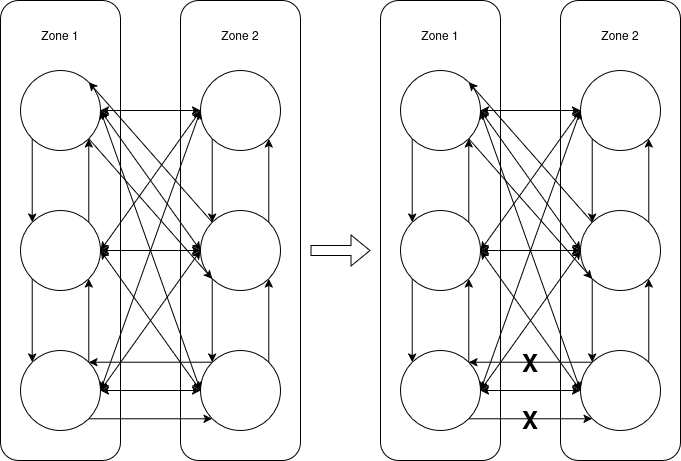
\includegraphics[height=8cm]{figures/setup-1.png}
    \caption{Network Topology for Setup 1}
    \label{fig:setup_1}
\end{figure}


\subsubsection{Unrestricted Connector Topology with Full Bidirectional Closure}
\label{sec:setup_2}

In this configuration, virtual centroids were connected to every physical intersection within their zones without capacity constraints. For bidirectional roads, both the forward and reverse directed edges were simultaneously removed from the network during testing. A visual representation of this is provided in Figure \ref{fig:setup_2}.

\begin{figure}[H]
    \centering
    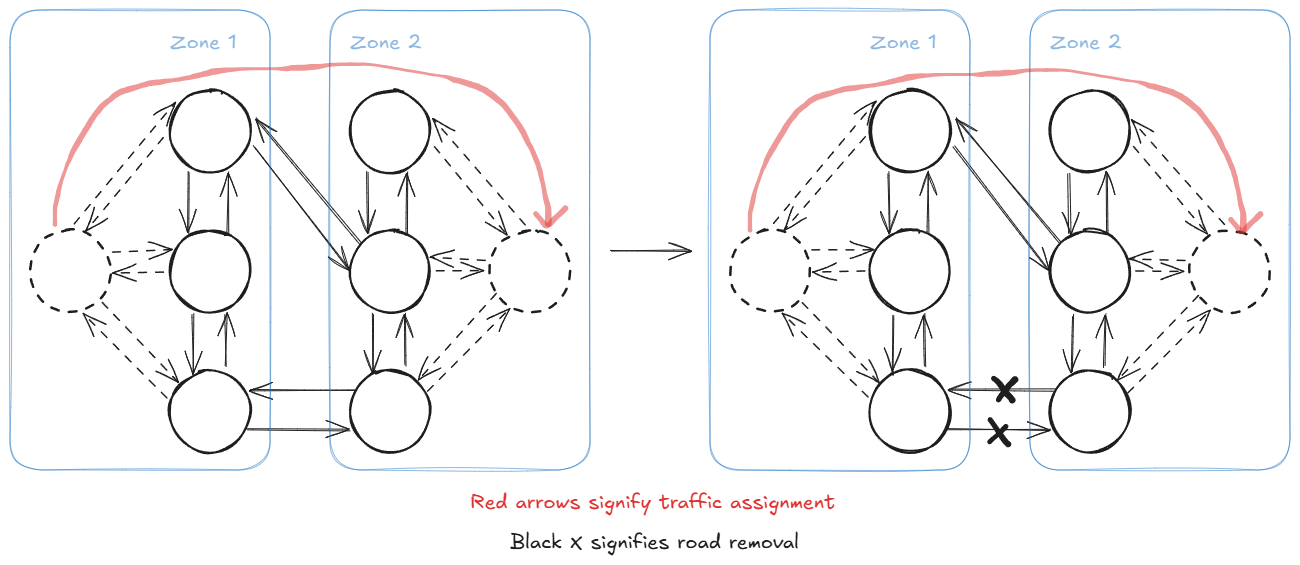
\includegraphics[width=13cm, height=7cm]{figures/setup-2.png}
    \caption{Network Topology for Setup 2}
    \label{fig:setup_2}
\end{figure}


\subsubsection{Connector Topology with Full Bidirectional Closure}
\label{sec:setup_3}

In this configuration, the number of nodes connected to the centroid are limited to certain nodes that have the highest volume based on the given AADT. For bidirectional roads, both the forward and reverse directed edges were simultaneously removed from the network during testing. A visual representation of this is provided in Figure \ref{fig:setup_3}.

\begin{figure}[H]
    \centering
    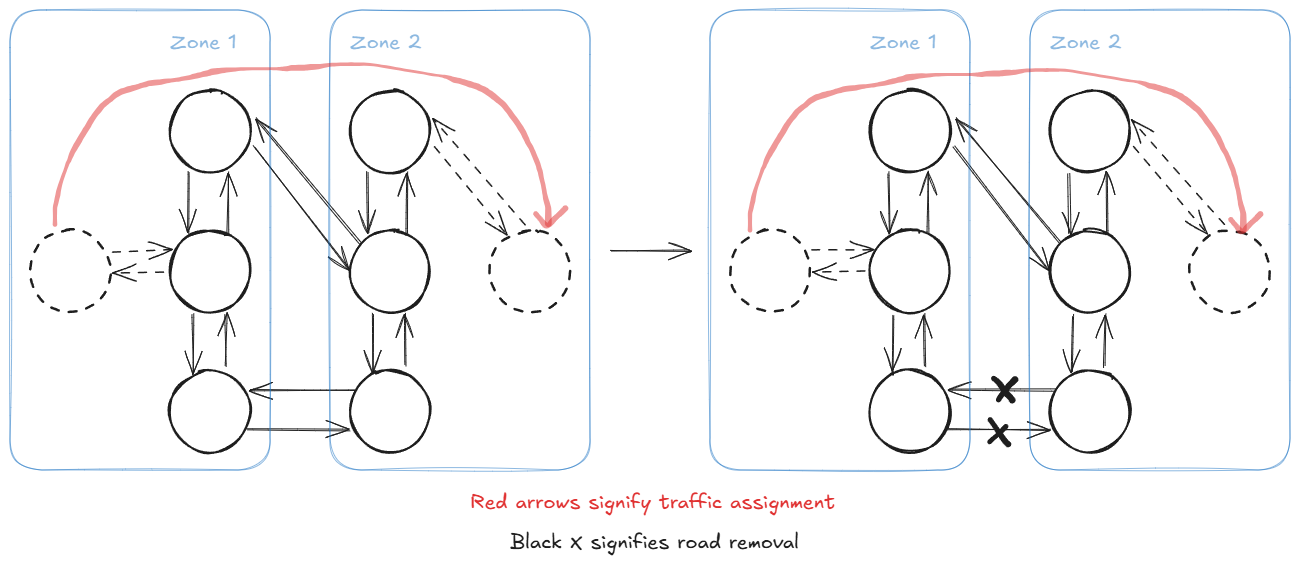
\includegraphics[width=13cm, height=7cm]{figures/setup-3.png}
    \caption{Network Topology for Setup 3.}
    \label{fig:setup_3}
\end{figure}

\subsubsection{Uniform Spatial Disaggregation with Unidirectional Closure}
\label{sec:setup_4}
In this configuration, demands were equally distributed across all physical nodes within a given zone. Unidirectional removals were executed uniformly across all tested segments, without caring if the baseline road was originally bidirectional or one way. A visual representation of this is provided in Figure \ref{fig:setup_4}.

\begin{figure}[H]
    \centering
    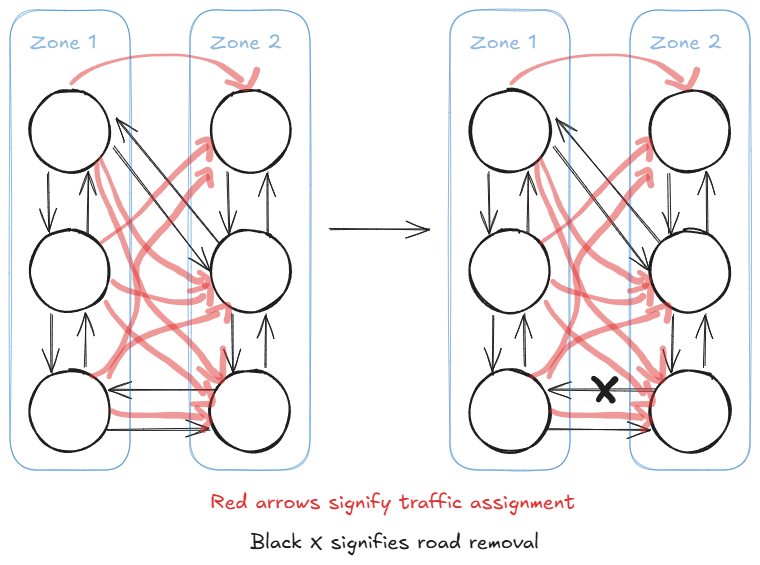
\includegraphics[height=8cm]{figures/setup-4.png}
    \caption{Network Topology for Setup 4.}
    \label{fig:setup_4}
\end{figure}


\subsubsection{Unrestricted Connector Topology with Unidirectional Closure}
\label{sec:setup_5}

In this configuration, virtual centroids were connected to every physical intersection within their zones without capacity constraints. A visual representation of this is provided in Figure \ref{fig:setup_5}.

\begin{figure}[H]
    \centering
    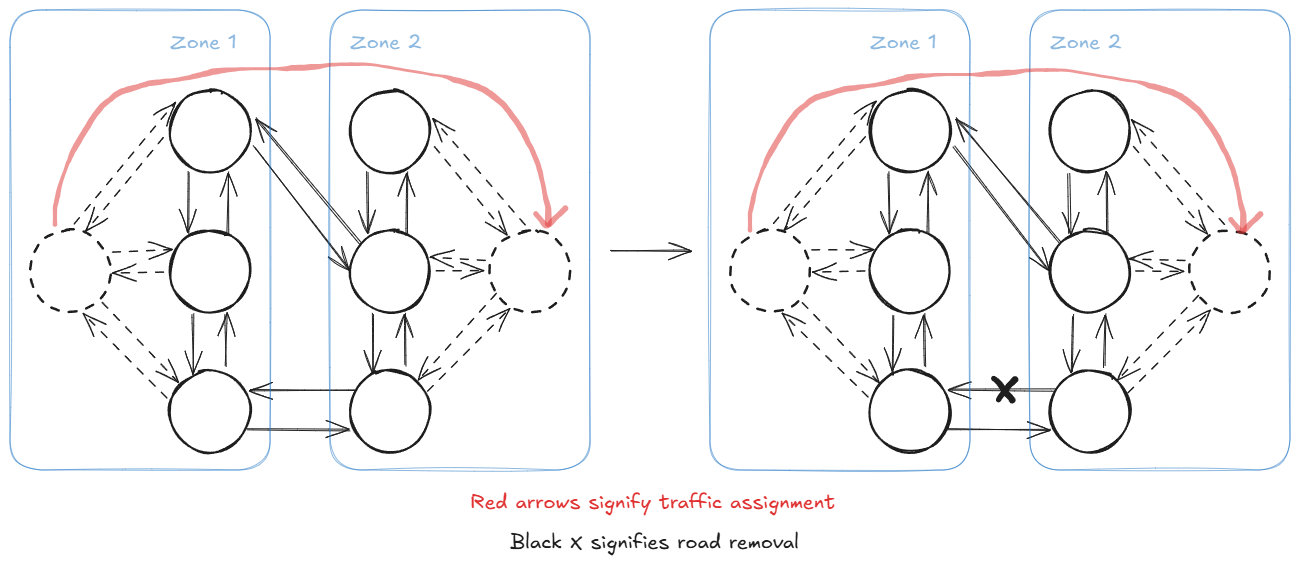
\includegraphics[width=13cm, height=7cm]{figures/setup-5.png}
    \caption{Network Topology for Setup 5.}
    \label{fig:setup_5}
\end{figure}

\subsubsection{Connector Topology with Unidirectional Closure}
\label{sec:setup_6}

In this configuration, the number of nodes connected to the centroid are limited to certain nodes that have the highest volume based on the given AADT. Unidirectional removals were executed uniformly across all tested segments, disregarding the baseline road's directionality. A visual representation of this is provided in Figure \ref{fig:setup_6}.

\begin{figure}[H]
    \centering
    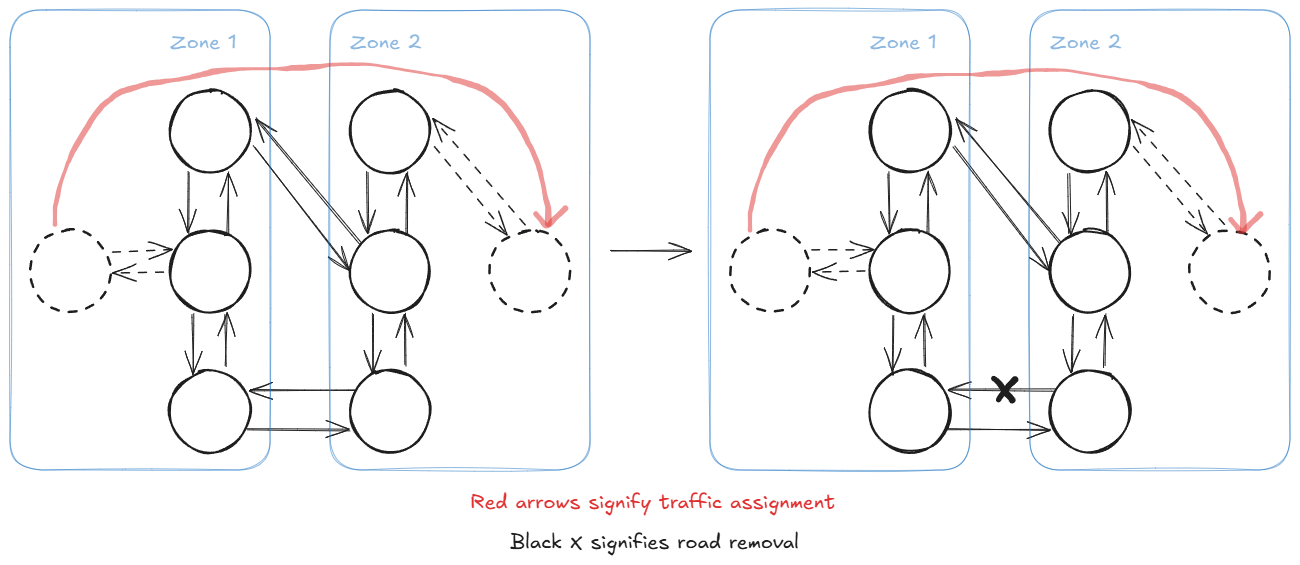
\includegraphics[width=13cm, height=7cm]{figures/setup-6.png}
    \caption{Network Topology for Setup 6.}
    \label{fig:setup_6}
\end{figure}
